\section{Relação Rastreamento e Reconhecimento}
\label{sec:rastreamento-reconhecimento}

	Até agora, foi mostrado como os Módulos de Rastreamento e de Reconhecimento funcionarão de maneira isolada, mas não como irão se relacionar. O Módulo de Rastreamento irá deter as informações sobre todos os usuários rastreados no ambiente e será responsável por requisitar reconhecimento ao Módulo de Reconhecimento, que deverá acontecer quando um novo usuário for detectado ou quando for necessário reconhecer um usuário já rastreado.

	Basicamente, quando um novo usuário for detectado, a relação entre rastreamento e reconhecimento acontecerá de acordo com as seguintes etapas e representada na Figura~\ref{fig:rastreamento-reconhecimento}:

		\begin{figure}[hbt]
			\begin{center}
				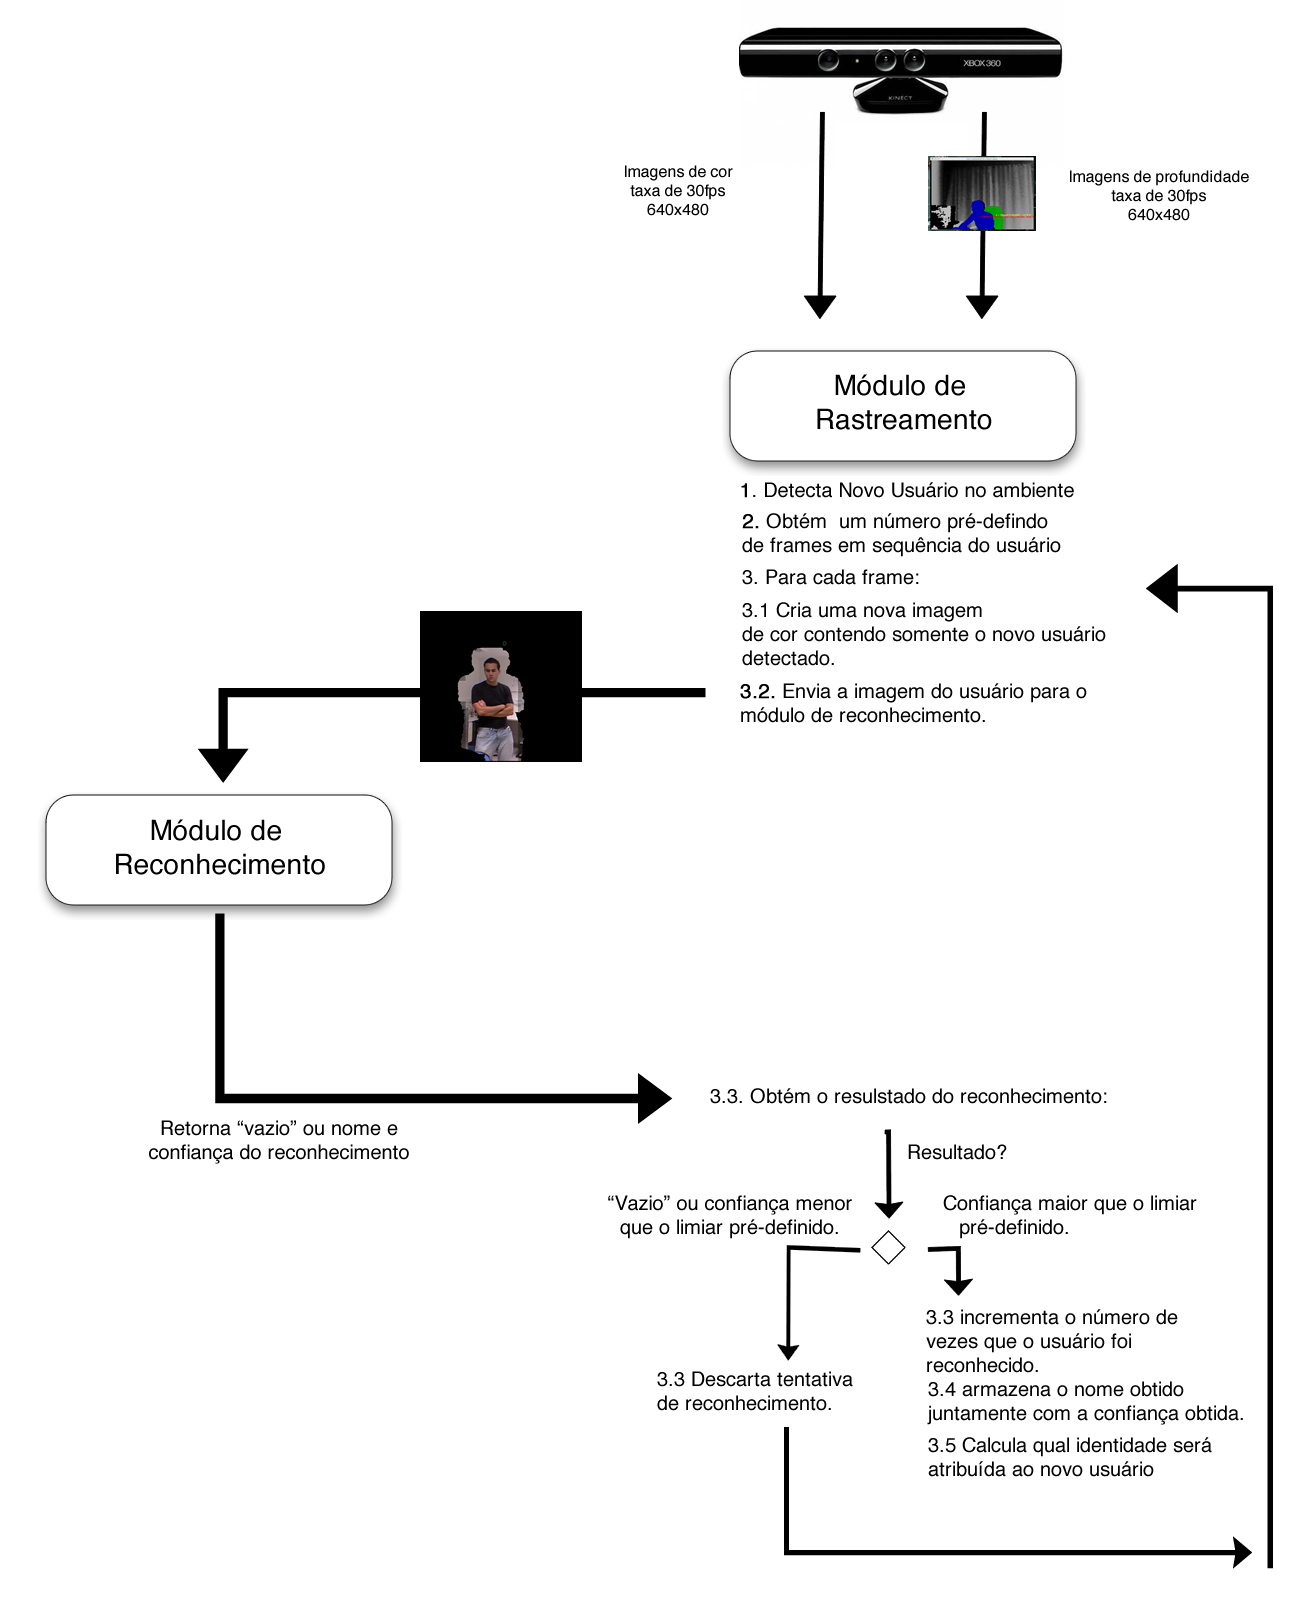
\includegraphics[scale=1.5]{figuras/4.ProblemaEProposta/esquema-tracker-reco.png}
			\end{center}
			\caption{Representação da relação que o Módulo de Rastreamento terá com o Módulo de Reconhecimento quando um novo usuário for detectado.}
			\label{fig:rastreamento-reconhecimento}
		\end{figure}
	
		\begin{enumerate}
		 	\item O Módulo de Rastreamento detecta novo usuário, e obtém um número pré-definido de imagens sucessivas do novo usuário. Para cada imagem, ele cria uma nova imagem de cor contendo somente aquele usuário, como mostrado na Figura (\textbf{colocar a figura aqui}), e a envia para o Módulo de Reconhecimento.
		 	\item Para cada imagem recebida, o Módulo de Reconhecimento tenta reconhecer o novo usuário e retorna ``vazio'' ou o nome e a confiança do reconhecimento.
		 	\item O Módulo de Rastreamento verifica se a confiança é maior que um limiar pré-definido, se for ele incrementa o contador que armazena o número de vezes que o usuário foi reconhecido, armazena o nome obtido juntamente com a confiança e calcula qual nome  será atribuído ao novo usuário. Esse cálculo será feito por meio de uma média ponderada utilizando os diferentes resultados obtidos por cada reconhecimento e suas respectivas confianças.
	 	\end{enumerate} 
	
	Ao invés de tentar realizar o reconhecimento somente quando novos usuários são detectados, o sistema \textit{True} continuará a tentar reconhecer os usuários já reconhecidos para melhorar a confiança no reconhecimento. Essas tentativas de reconhecer novamente os usuários ocorrerão em intervalos de tempo pré-definidos seguindo as mesmas etapas de quando um novo usuário for detectado. A única etapa que será diferente será a primeira: ao invés de obter várias imagens de um mesmo usuário, serão obtidas uma imagem de cada usuário rastreado e as mesmas serão enviadas ao Módulo de Reconhecimento.

	Desta maneira, o Módulo de Rastreamento conseguirá reunir em um só lugar todas as informações sobre os usuários rastreados, como localização corrente, nome, confiança do reconhecimento, quantas vezes o usuário foi reconhecido e quais diferentes nomes foi atribuído ao mesmo.